\documentclass[a4paper,11pt]{article}
\usepackage{latexsym}
\usepackage{xcolor}
\usepackage{float}
\usepackage{ragged2e}
\usepackage{wrapfig}
\usepackage{lipsum}
\usepackage{tabularx}
\usepackage{titlesec}
\usepackage{geometry}
\usepackage{marvosym}
\usepackage{verbatim}
\usepackage{enumitem}
\usepackage[hidelinks]{hyperref}
\usepackage{fancyhdr}
\usepackage{fontawesome5}
\usepackage{multicol}
\usepackage{graphicx}
\usepackage{array}
\usepackage[T1]{fontenc}
\setlength{\footskip}{4.08003pt} 
\pagestyle{fancy}
\fancyhf{} % clear all header and footer fields
\fancyfoot{}
\renewcommand{\headrulewidth}{0pt}
\renewcommand{\footrulewidth}{0pt}
\geometry{left=1.4cm, top=1cm, right=1.4cm, bottom=1cm}
% Adjust margins
%\addtolength{\oddsidemargin}{-0.5in}
%\addtolength{\evensidemargin}{-0.5in}
%\addtolength{\textwidth}{1in}
\urlstyle{same}

\raggedright
\setlength{\footskip}{4.08003pt}

% Sections formatting
\titleformat{\section}{
  \vspace{-8pt}\scshape\raggedright\large
}{}{0em}{}[\color{black}\titlerule \vspace{-6pt}]

%-------------------------
% Custom commands
\newcommand{\resumeItem}[2]{
  \item{
    \textbf{#1}{\hspace{0.5mm}#2 \vspace{-0.5mm}}
  }
}

\newcommand{\resumePOR}[3]{
\vspace{0.5mm}\item
    \begin{tabular*}{0.97\textwidth}[t]{l@{\extracolsep{\fill}}r}
        \textbf{#1}\hspace{0.3mm}#2 & \textit{\small{#3}} 
    \end{tabular*}
    \vspace{-2mm}
}

\newcommand{\resumeSubheading}[4]{
\vspace{0.5mm}\item
    \begin{tabular*}{0.98\textwidth}[t]{l@{\extracolsep{\fill}}r}
        \textbf{#1} & \textit{\footnotesize{#4}} \\
        \textit{\footnotesize{#3}} &  \footnotesize{#2}\\
    \end{tabular*}
    \vspace{-2.4mm}
}

\newcommand{\resumeProject}[4]{
\vspace{0.5mm}\item
    \begin{tabular*}{0.98\textwidth}[t]{l@{\extracolsep{\fill}}r}
        \textbf{#1} & \textit{\footnotesize{#3}} \\
        \footnotesize{\textit{#2}} & \footnotesize{#4}
    \end{tabular*}
    \vspace{-2.4mm}
}

\newcommand{\resumeSubItem}[2]{\resumeItem{#1}{#2}\vspace{-4pt}}

% \renewcommand{\labelitemii}{$\circ$}
\renewcommand{\labelitemi}{$\vcenter{\hbox{\tiny$\bullet$}}$}

\newcommand{\resumeSubHeadingListStart}{\begin{itemize}[leftmargin=*,labelsep=0mm]}
\newcommand{\resumeHeadingSkillStart}{\begin{itemize}[leftmargin=*,itemsep=1.7mm, rightmargin=2ex]}
\newcommand{\resumeItemListStart}{\begin{justify}\begin{itemize}[leftmargin=3ex, rightmargin=2ex, noitemsep,labelsep=1.2mm,itemsep=0mm]\small}

\newcommand{\resumeSubHeadingListEnd}{\end{itemize}\vspace{0.5mm}}
\newcommand{\resumeHeadingSkillEnd}{\end{itemize}\vspace{-2mm}}
\newcommand{\resumeItemListEnd}{\end{itemize}\end{justify}\vspace{-4mm}}
\newcolumntype{L}{>{\raggedright\arraybackslash}X}%
\newcolumntype{R}{>{\raggedleft\arraybackslash}X}%
\newcolumntype{C}{>{\centering\arraybackslash}X}%
%---- End of Packages and Functions ------

%-------------------------------------------
%%%%%%  CV STARTS HERE  %%%%%%%%%%%
%%%%%% DEFINE ELEMENTS HERE %%%%%%%
\newcommand{\name}{JI Zhuangzhi}
% \newcommand{\emaila}{your@email.com}
\newcommand{\emailb}{zhuangzhiji@outlook.com}
\newcommand{\course}{Artificial Intelligence}


\begin{document}
\fontfamily{cmr}\selectfont

%----------HEADING-----------------
\parbox{2.6cm}{%
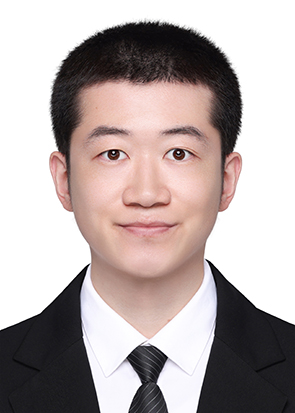
\includegraphics[width=2.35cm,clip]{andrew.jpg}
}
\parbox{\dimexpr\linewidth-2.9cm\relax}{
\begin{tabularx}{\linewidth}{L r} \\
  \textbf{\Large \name} & {\raisebox{0.0\height}{\footnotesize \faPhone}\ +33 7 67 68 91 96}\\
    \empty &  \href{mailto:\emailb}{\raisebox{0.0\height}{\footnotesize \faEnvelope}\ {\emailb}}\\
   \empty & \href{https://github.com/Andrew-Dylan}{\raisebox{0.0\height}{\footnotesize \faGithub}\ {github.com/Andrew-Dylan}} \\
\end{tabularx}}


%-----------EDUCATION-----------
\section{\textbf{Formation}}
\resumeSubHeadingListStart
    % Cycle master
    \resumeSubheading
        {Tiangong University}{Tianjin, Chine}
        {École d'intelligence artificielle}{Septembre 2023 -- Juin 2026}
    \resumeItemListStart
        \item{\textbf{Spécialité :} Intelligence artificielle}
        \item \textbf{Cours pertinents :} Apprentissage profond, vision par ordinateur, traitement d'images et reconnaissance des formes
    \resumeItemListEnd
    
    % Cycle licence
    \resumeSubheading
        {Shanxi Datong University}{Datong, Chine}
        {Collège d'informatique et d'ingénierie des réseaux}{Septembre 2019 -- Juin 2023}
    \resumeItemListStart
         \item{\textbf{Spécialité :} Sciences et technologies de l'informatique}
         \item \textbf{Cours pertinents :} structures de données, systèmes d'exploitation, systèmes de gestion de bases de données.
    \resumeItemListEnd
\resumeSubHeadingListEnd


%-----------Publication----------------
\section{\textbf{Publications}}
\resumeSubHeadingListStart
    \item Tang, Chunming, et \textbf{Ji, Zhuangzhi}. "Dynamic Sparse Attention and Frequency-Spatial Complementary Network for SAR Ship Detection." \textit{IEEE Geoscience and Remote Sensing Letters}, 2026 \textbf{(Accepté)}
    \item Tang, Chunming, et \textbf{Ji, Zhuangzhi}. "IRS-DETR: Efficient Infrared Ship Detection Transformer for Complex Sea-Air Backgrounds." \textit{IEEE Geoscience and Remote Sensing Letters}, 2025 \textbf{(JCR Q1)}
\resumeSubHeadingListEnd


%-----------Research Experience-----------------
\section{\textbf{Expérience de recherche}}
\resumeSubHeadingListStart
    \resumeSubheading
        {École d'intelligence artificielle, Tiangong University}
        {Tianjin, Chine}
        {Étudiant-chercheur en master}{Septembre 2023 -- Juin 2026}
        \resumeItemListStart
        
        \item Développement d'une application de traitement d'images et de reconnaissance des formes en Python, intégrant des fonctions clés telles que le filtrage, la transformation et l'extraction de caractéristiques visuelles, couvrant l'ensemble du processus de traitement d'images.
        
        \item Conception et mise en œuvre d'un modèle léger de perception infrarouge maritime, améliorant de 3,6 \% la précision dans la détection des petites cibles par rapport aux méthodes de référence, tout en conservant des performances en temps réel.
        
        \item Gestion du traitement de bout en bout d'un jeu de données de télédétection infrarouge pour l'entraînement et la validation des modèles ; rédaction des sections méthodologique et expérimentale de l'article qui en a résulté, publié dans \textit{\textbf{IEEE Geoscience and Remote Sensing Letters}}.

        \item Ces travaux m'ont permis d'acquérir une solide expérience en vision par ordinateur et en détection d'objets, que je souhaite maintenant appliquer à la perception multimodale et à la simulation immersive dans le cadre de mon projet de thèse.
        \resumeItemListEnd
\resumeSubHeadingListEnd


%-----------INTERNSHIP EXPERIENCE-----------------
% \section{\textbf{Internship Experience}}
% \resumeSubHeadingListStart
% \resumeSubheading
%     {Momenta.ai}{Shanghai, China}
%     {Road Test Intern}{Nov 2025 - Dec 2025} 
% \resumeItemListStart
%     \item {High-fidelity testing for L2/L3 Advanced Driver Assistance Systems in complex urban and highway scenarios.}
%     \item {Conducted targeted data collection, successfully capturing critical edge cases like queue cut-in and urban merging.}
%     \item {Collaborated with perception and planning teams to diagnose system failures identified during rigorous road tests, providing structured feedback for rapid algorithm iteration.}
% \resumeItemListEnd

% \resumeSubheading
%         {Pony.ai}{Beijing, China}
%         {Autonomous Driving Road Test Intern}{Dec 2024 - Mar 2025} 
% \resumeItemListStart
%         \item {Diagnosed perception model failures by analyzing tera-scale LiDAR point cloud and camera data, identifying and categorizing over 100 critical edge cases related to adverse weather and dense traffic scenarios.}
%         \item {Collaborated with the perception team to implement and test new algorithms, utilizing C++ and Python in a Linux environment.}
% \resumeItemListEnd
% \resumeSubHeadingListEnd

%-----------THESIS PROJECT-----------------
% \section{\textbf{Projet de thèse}}
% \begin{itemize}[leftmargin=0.15in, itemsep=2pt]
%     \item \textbf{Titre provisoire :} Écosystèmes cyclables intelligents : reconnaissance d'intention, prédiction de trajectoire et simulation immersive
%     \item \textbf{Mots-clés :} MARL, XAI, SUMO, CARLA, VR, ITS
%     \item \textbf{Objectif :} Développer un cadre combinant optimisation d'infrastructure, navigation adaptative et simulation immersive pour améliorer la sécurité des cyclistes en milieu urbain connecté.
% \end{itemize}

%-----------RESEARCH INTERESTS-----------------
\section{\textbf{Domaines de recherche}}
\begin{itemize}[leftmargin=0.15in, itemsep=2pt]
    \item Systèmes de transport intelligents, simulation du trafic, perception multimodale, vision par ordinateur, compréhension de scènes
\end{itemize}

%-----------Technical skills-----------------
\section{\textbf{Compétences techniques}}
\begin{itemize}[leftmargin=0.15in, itemsep=2pt]
    \item \textbf{Langages de programmation :} Python, C/C++
    \item \textbf{Frameworks et bibliothèques :} PyTorch, OpenCV, Pandas, NumPy
    \item \textbf{Outils et environnements :} Git, Linux, Docker, Shell 
\end{itemize}

%-------------------------------------------
\end{document}
